\subsubsection{Descripci\'on} 

% \textbf{Motivation
% D-basis: Ordered direct implicational basis of a finite closure system, K. Adaricheva, et.al., Discrete Applied Mathematics, 161 (6): 707-723, 2013
% Compromise between the size of the implicational set and the efficiency of its management
% }

Este algoritmo se desarroll\'o por E. Rodr\'iguez-Lorenzo et al. en \cite{DBasis} con el objetivo  de reducir el coste computacional del c\'alculo del cierre haciendo uso del concepto de D-Base presentado por K. Adaricheva \cite{Adaricheva}.\\

\IncMargin{1em}
\begin{algorithm}[H]
    \SetKwFunction{Add}{Add}
    \SetKwFunction{MinimalCovers}{MinimalCovers}
    \SetKwFunction{MinGen}{$MinGen_{0}$}
    \SetKwFunction{OrderedComp}{OrderedComp}
    \SetAlgoLined
    % \LinesNumbered
    \DontPrintSemicolon
    \SetKw{KwOr}{or}
    \KwIn{ 
        $\Sigma$, an implicational system on $M$ 
    }
    \KwOut{The D-basis $ \Sigma_{D} $ on $M$}
    \Begin{
        \ $MinGen = \MinGen{$M, \ \Sigma $}$\;
        \ $C := \emptyset$\;
        \ForEach{$\langle a,mg(C)\rangle \in MinGen $}{
            \ForEach{$a \in C $}{
                \ $C := \Add{$\langle a,mg(C)\rangle,C$}$
            }
        }
        \ $\Sigma_{D} := \emptyset$ \;
        \ForEach{$\langle a,mg_{a}\rangle \in C $}{
            \ $mg_{a} := \MinimalCovers{$mg_{a}$}$\;
            \ForEach{$g \in ,mg_{a} $}{
                $\Sigma_{D} : = \Sigma_{D} \cup \{g \to a\}$
            }
        }
        \OrderedComp{$\Sigma_{D}$}\;
        \Return $\Sigma_{D}$
    }%end beginre
    \caption{D-basis algorithm}\label{alg:7}
\end{algorithm}\DecMargin{1em}
\bigskip

Antes de entrar en el concepto de D-Base, se detallar\'an otros conceptos con el fin de entrar en contexto.\\

Se parte de un conjunto de implicaciones, \( \Sigma \), y un conjunto de atributos \( M \).\\

\textbf{Operador de cierre at\'omico}\\
Se parte de que \(\Sigma\) cumple las siguientes propiedades:
\begin{itemize}
    \item \(\oslash^+_{\Sigma} = \oslash\), es decir, el cierre del vac\'io con respecto a \(\Sigma\) es el vac\'io.
    \item \(\forall x,y \in M, \{x\}^+_{\Sigma} = \{y\}^+_{\Sigma} \implies x = y\)
\end{itemize}
Se define el operador de cierre at\'omico como: 
\begin{center}
    \((-)^*_{\Sigma}::2^M \to 2^M \) \\
    \(X^*_{\Sigma} = \cup_{\substack{x \in X}} \{x\}^+_{\Sigma}, \ \forall \ X \subseteq M \)
\end{center}


\textbf{Covers}\\
Sea \(X \subseteq M\) y \(x \in X\), se dice que \(X\) es un cover de \(x\) si \(x \in X^+_{\Sigma} \setminus X\), denotado por \(x \sim X\)

\textbf{Propers covers} \\
Sea \(X \subseteq M\) y \(x \in X\), se dice que \(X\) es un proper cover de \(x\) si \(x \in X^+_{\Sigma} \setminus X^*_{\Sigma}\), denotado por \(x \dot\sim X\)

\textbf{Minimals propers covers}\\
Sea \(X \subseteq M\) y \(x \in X\), se dice que \(X\) es un minimal proper cover de \(x\) si se cumple que:
\begin{itemize}
    \item \(x \dot\sim X\)
    \item \(x \dot\sim Z\) y \(Z \subseteq X^*_{\Sigma} \implies X \subseteq Z\)
\end{itemize}

\textbf{D-Base}\\
Podemos definir la D-Base para \(\Sigma\) como el par \(<\Sigma_a, \Sigma_n>\), donde:

\begin{itemize}
    \item \(\Sigma_a = \{y \to x | y \in M, x \in X^+_{\Sigma}, x \neq y \} \)
    \item \(\Sigma_n = \{X \to x | X \subseteq M, x \in X, X \ minimal \ proper \ cover \ de \ x\} \)

\end{itemize}

\textbf{Teorema}(\cite{Adaricheva})\\
Sea \(\Sigma\) un sistema implicacional. Si \(<\Sigma_a, \Sigma_n>\) es D-Base de \(\Sigma\) y \(\Sigma_d = \Sigma_a\cup \Sigma_n\) de forma que las implicaciones de \(\Sigma_a\) aparecen antes que las de \(\Sigma_n\), entonces \(\Sigma_d\) es una base ordenada directa de forma que \(\Sigma_d \equiv \Sigma\).

De este teorema radica la importancia de tener un algoritmo para el c\'alculo de la D-Base de un sistema implicacional \(\Sigma\), ya que a partir de esta, se podr\'a obtener una base ordenada directa, que como ya se ha dicho con anterioridad, permite que el c\'alculo del cierre de \(\Sigma\) sea mucho m\'as r\'apido y eficiente.\\


\newpage 
\subsubsection{C\'odigo} 
\lstinputlisting{r_code/d.basis.R}
\newpage
\subsubsection{Ejemplo}
A continuaci\'on se muestra un peque\~no ejemplo de ejecuci\'on del algoritmo. Para ello se parte del conjunto de atributos \(M\) y del conjunto de implicaciones \(\Gamma\) que se puede ver en la imagen \ref{fig:dbasis_2}.
\begin{figure}[H]
    \centering
    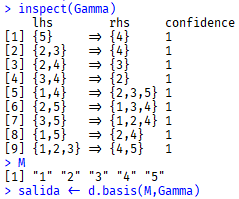
\includegraphics[scale=1]{dbasis_2}
    \caption{Ejemplo D-Base 1}
    \label{fig:dbasis_2}
\end{figure} 
Aqu\'i se puede ver el resultado:
\begin{figure}[H]
    \centering
    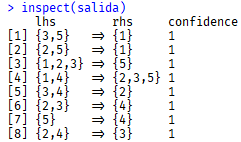
\includegraphics[scale=1]{dbasis_3}
    \caption{Ejemplo D-Base 2}
    \label{fig:dbasis_3}
\end{figure} 
Aunque el ejemplo expuesto tiene un conjunto reducido de implicaciones y atributos, se puede apreciar la mejora de rendimiento a la hora del c\'alculo del cierre si se hace sobre una base, en comparaci\'on a si se hace con el conjunto de implicaciones inicial.
\begin{figure}[H]
    \centering
    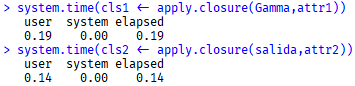
\includegraphics[scale=1]{dbasis_4}
    \caption{Comparativa de c\'alculo del cierre}
    \label{fig:dbasis_4}
\end{figure} 

Teniendo en cuenta que existen problemas en los que se requieren el c\'alculo masivo de cierres, cualquier peque\~na mejora puede suponer una reducci\'on de tiempo y recursos necesarios considerable.